%----------------------------------------------------------------------------------------
%	PACKAGES AND OTHER DOCUMENT CONFIGURATIONS
%----------------------------------------------------------------------------------------

\documentclass[titlepage]{article}

\usepackage{fancyhdr} % Required for custom headers
\usepackage{lastpage} % Required to determine the last page for the footer
\usepackage{extramarks} % Required for headers and footers
\usepackage{graphicx} % Required to insert images
\usepackage{pdflscape} % Allow us to make certain pages in landscape orientation
\usepackage{amsmath} % Allow multiple line equations
\usepackage{amssymb}
\usepackage{scrextend}
\usepackage{xcolor}
\usepackage{listings} 
\usepackage{dirtree}
\usepackage[numbers]{natbib} 

\definecolor{mGreen}{rgb}{0,0.6,0}
\definecolor{mGray}{rgb}{0.5,0.5,0.5}
\definecolor{mPurple}{rgb}{0.58,0,0.82}
\definecolor{backgroundColour}{rgb}{0.95,0.95,0.92}

\lstdefinestyle{CStyle}{
	backgroundcolor=\color{backgroundColour},   
	commentstyle=\color{mGreen},
	keywordstyle=\color{magenta},
	numberstyle=\tiny\color{mGray},
	stringstyle=\color{mPurple},
	basicstyle=\footnotesize,
	breakatwhitespace=false,         
	breaklines=true,                 
	captionpos=b,                    
	keepspaces=true,                 
	numbers=none,                   
	numbersep=5pt,                  
	showspaces=false,                
	showstringspaces=false,
	showtabs=false,                  
	tabsize=4,
	language=C
}

\lstdefinestyle{CStyleInline}{
	backgroundcolor=\color{white},   
	commentstyle=\color{mGreen},
	keywordstyle=\color{magenta},
	numberstyle=\tiny\color{mGray},
	stringstyle=\color{mPurple},
	basicstyle=\footnotesize,
	breakatwhitespace=false,         
	breaklines=true,                 
	captionpos=b,                    
	keepspaces=true,                 
	numbers=none,                   
	numbersep=5pt,                  
	showspaces=false,                
	showstringspaces=false,
	showtabs=false,                  
	tabsize=2,
	language=C
}

% Margins
\topmargin=-0.45in
\evensidemargin=0in
\oddsidemargin=0in
\textwidth=6.5in
\textheight=9.0in
\headsep=0.25in 

\linespread{1.1} % Line spacing

% Set up the header and footer
\pagestyle{fancy}
\lhead{CAB403}
\chead{Distributed Systems Major Assignment}
\rhead{Pedro Alves (n9424342)}
\lfoot{\lastxmark} % Bottom left footer
\cfoot{} % Bottom center footer
\rfoot{Page\ \thepage\ of\ \pageref{LastPage}} % Bottom right footer
\renewcommand\headrulewidth{0.4pt} % Size of the header rule
\renewcommand\footrulewidth{0.4pt} % Size of the footer rule

\setlength\parindent{0pt} % Removes all indentation from paragraphs

%----------------------------------------------------------------------------------------
%	DOCUMENT STRUCTURE COMMANDS
%----------------------------------------------------------------------------------------

\setcounter{secnumdepth}{0} % Removes default section numbers
   
%----------------------------------------------------------------------------------------
%	NAME AND CLASS SECTION
%----------------------------------------------------------------------------------------

\newcommand{\Title}{Distributed Systems Major Assignment} % Assignment title
\newcommand{\DueDate}{26 October 2018} % Due date
\newcommand{\Class}{CAB403 Systems Programming} % Course/class
\newcommand{\AuthorName}{Pedro Alves (n9424342)} 

%----------------------------------------------------------------------------------------
%	TITLE PAGE
%----------------------------------------------------------------------------------------

\title{
\vspace{2in}
\textmd{\huge\textbf{\Class}}\\
\textmd{{\Title}}\\
\vspace{3in}
\textmd{{\AuthorName}}
}
\author{}

%----------------------------------------------------------------------------------------

\begin{document}

\maketitle
\clearpage

%----------------------------------------------------------------------------------------
%	STATEMENT OF COMPLETENESS
%----------------------------------------------------------------------------------------
\section{Statement of completeness}

%----------------------------------------------------------------------------------------
%	STATEMENT OF COMPLETENESS
%----------------------------------------------------------------------------------------
All tasks outlined in the assignment brief were completed with no deviations from the specification. I performed extensive testing and did not find any problems or deficiencies with my solution. 
\\
I chose to complete this project individually. All work is my own.

%----------------------------------------------------------------------------------------
%	COMPILATION INSTRUCTIONS
%----------------------------------------------------------------------------------------
\section{Compilation Instructions}

%----------------------------------------------------------------------------------------
%	COMPILATION INSTRUCTIONS
%----------------------------------------------------------------------------------------
The project directory when the folder is unzipped should have the following structure:
\\
\dirtree{%
	.1 root.
	.2 bin.
	.3 Authentication.txt.
	.2 doc.
	.3 AssignmentBrief.pdf.
	.3 n9424342\_CAB403\_Report.pdf.
	.2 src.
	.3 client.c.
	.3 server.c.
	.3 leaderboard.h.
	.3 leaderboard.c.
	.3 message.h.
	.3 message.c.
	.3 minesweeper.h.
	.3 minesweeper.c.
	.2 Makefile.
}
\ \\
The program can be compiled by opening a terminal window at the \emph{root} of the folder and then typing the command \emph{make all}.
\\
Two \emph{.exe} files called \textit{server} and \textit{client} should be created in the \emph{root/bin} directory. 

%----------------------------------------------------------------------------------------
%	PROGRAM LAUNCH INSTRUCTIONS
%----------------------------------------------------------------------------------------
\section{Program Launch Instructions}

%----------------------------------------------------------------------------------------
%	PROGRAM LAUNCH INSTRUCTIONS
%----------------------------------------------------------------------------------------
Open a terminal at the \textit{root/bin} directory. The server and clients can be launched as follows.
\subsection{Server}
\begin{lstlisting}[language=bash]
$ ./server
\end{lstlisting}
Will open a server on port 12345.
\begin{lstlisting}[language=bash]
$ ./server portnum
\end{lstlisting}
Will open a server on the port given by the number \textit{portnum}.
\\
\subsection{Client}
\begin{lstlisting}[language=bash]
$ ./client server_ip_address portnum
\end{lstlisting}
Will open a client which will attempt to connect to a server at the address \textit{server\_ip\_address} on port \textit{port\_num}.
\begin{lstlisting}[language=bash]
$ ./client 127.0.0.1 portnum
$ ./client localhost portnum
\end{lstlisting}
Both are valid when connecting to a server on the local network. 

\clearpage

%----------------------------------------------------------------------------------------
%	REPRESENTING THE PLAYFIELD
%----------------------------------------------------------------------------------------
\section{Representing the Playfield}

%----------------------------------------------------------------------------------------
%	REPRESENTING THE PLAYFIELD
%----------------------------------------------------------------------------------------
The playfield is represented as a two-dimensional array of \textit{Tile} objects. 
\begin{lstlisting}[style=CStyle]
// minesweeper.h: Line 26
Tile field[FIELD_WIDTH][FIELD_HEIGHT];
\end{lstlisting}
Each \textit{Tile} object is a struct that holds information that helps control the game.
\begin{lstlisting}[style=CStyle]
// minesweeper.h: Lines 15-20
typedef struct {
	int adjacent_mines;
	int revealed;
	int has_mine;
	int has_flag;
} Tile;
\end{lstlisting}
A two-dimensional array was chosen to save programming time. The ability to access the field directly through \textit{x-y} coordinates (\lstinline{field[x][y]}) greatly increases readability of the program. 
\\
There is some increased computational complexity to iterate through the field when compared with a one-dimensional array but since the field only contains 81 tiles, it's not enough of a drawback to sacrifice program readability. 

%----------------------------------------------------------------------------------------
%	LEADERBOARD
%----------------------------------------------------------------------------------------
\section{Leaderboard}

%----------------------------------------------------------------------------------------
%	LEADERBOARD
%----------------------------------------------------------------------------------------
The leaderboard was implemented through the use of data structures that can represent the tables shown below. \textbf{Username} is an unique id on the \textit{User Records} table but not on \textit{Games Won}.
\\
\\
User Records: 
\begin{tabular}{|c|c|c|}
	\hline
	\textbf{Username}&Games Won&Games Played\\
	\hline
\end{tabular}
\quad
Games Won: 
\begin{tabular}{|c|c|}
	\hline
	\textbf{Username}&Time Taken\\
	\hline
\end{tabular}
\\
\\
When a client requests the leaderboard, the \textit{Games Won} table will be printed to the terminal. User information (games played/won) will be added to each row by getting the data from the \textit{User Records} table that matches the \textbf{Username}. 
\\
The \textit{User Records} table was implemented as a Linked List with nodes consisting of \textit{user} structures. A HEAD and a TAIL pointer were created in order to access the list. 
\begin{lstlisting}[style=CStyle]
// leaderboard.h: Lines 11-16
struct user {
	char* username;         
	int games_won;
	int games_played;     
	struct user* next; // Pointer to the next user
};

// leaderboard.c: Lines 12-13
struct user* head_userinfo = NULL;   // HEAD of the linked list of the user details
struct user* tail_userinfo = NULL;   // TAIL of the linked list of the user details
\end{lstlisting}
The \textit{Games Won} table was also implemented as a Linked List but used nodes consisting of \textit{game} structures.
\begin{lstlisting}[style=CStyle]
// leaderboard.h: Lines 22-26
	struct game {
	char* username; 
	int time_taken;       
	struct game* next;   // Pointer to the next game completed
};

// leaderboard.c: Lines 15-16
struct game* head_gameinfo = NULL;   // HEAD of the linked list of the queue of clients
struct game* tail_gameinfo = NULL;   // TAIL of the linked list of the queue of clients
\end{lstlisting}
In order to choose the data structure that will be used to represent the leaderboard, the required operations to be completed on the structure were first written down. 
\\
The most common operation will be \textit{search} followed by \textit{insert}. In some cases \textit{access} might be used and there is also no need to have functionality for a \textit{delete} operation. 
\\
Several data structures were considered and their time complexities for the required operations were written down.
\begin{center}
\begin{tabular}{|c|c|c|c|c|c|c|}
	\cline{1-7}
	& \multicolumn{3}{|c|}{Average} & \multicolumn{3}{|c|}{Worst Case}	\\
	\cline{1-7}
	Data Structure & Search & Insertion & Access & Search & Insertion & Access \\
	\hline
	Array				& O(n)	& O(n)	& O(1)	& O(n)	& O(n)	& O(1)	\\
	Singly-Linked List	& O(n)	& O(1)	& O(n)	& O(n)	& O(1)	& O(n)	\\
	Hash Table			& O(1)	& O(1)	& N/A	& O(n)	& O(n)	& N/A	\\
	Red-Black Tree		& O(logn) & O(logn) & O(logn) & O(logn) & O(logn) & O(logn) \\
	\hline
\end{tabular}
\end{center}
Initally, a Red-Black tree was going to be used. However, the extra complexity it would add for a programmer to read/debug and the extra time it would take to implement is not worth the small gains in computational efficiency. 
\\ 
As the leaderboard is wiped whenever the server shuts down, \textit{n} has a low chance of reaching a large enough value where the extra efficiency from a Red-Black Tree will be felt.
\\
A Singly-Linked List was chosen in the end as it is the simplest data structure that could've been implemented (as a Linked List was already in use for the client queue) while providing good efficiency for the most used operations. 
\begin{figure} [!ht]
	\centering
	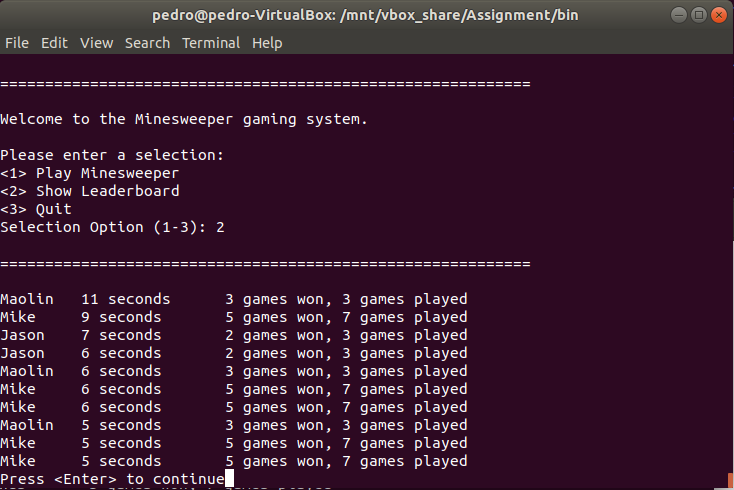
\includegraphics[width=1\textwidth]{images/Leaderboard} 
	\caption{The leaderboard with examples of how it is sorted and displayed}
	\label{fig:leaderboard} 
\end{figure}

\clearpage

%----------------------------------------------------------------------------------------
%	HANDLING CRITICAL SECTION PROBLEMS
%----------------------------------------------------------------------------------------
\section{Handling Critical Section Problems}

%----------------------------------------------------------------------------------------
%	HANDLING CRITICAL SECTION PROBLEMS
%----------------------------------------------------------------------------------------
With the addition of multi-threading, four critical section problems had to be solved in order to keep the threads synchronized and to prevent bugs.
\subsection{Using \textit{rand()}}
Whenever a Minesweeper game is initialized, the \textit{rand()} function is used to place the mines in the field. As \textit{rand()} is not thread-safe, a simple mutex lock was used.
\begin{lstlisting}[style=CStyle]
// server.c: Line 50
pthread_mutex_t rand_mutex = PTHREAD_MUTEX_INITIALIZER;

// server.c: Lines 587-615
void update_main_menu(...) {
	...
	switch(selection) {
		case 1:
			pthread_mutex_lock(&rand_mutex);
			minesweeper_init(sweeper_state);	// The rand() function is used here
			pthread_mutex_unlock(&rand_mutex);
			*state = PLAYING;
			break;
	...
}
\end{lstlisting}

\subsection{Performing I/O operations with text file}
The current implementation of the server does not write to the \textit{Authentication.txt} file. Therefore, initially, no mutex was going to be used as all access to the file would be read-only.
\\
After further research, it was found that opening a file that is already open leads to implementation-defined behavior \cite{fopen}.
\\
To be safe, a simple mutex lock to restrict access to the file was implemented.
\begin{lstlisting}[style=CStyle]
// server.c: Line 47
pthread_mutex_t file_read_mutex = PTHREAD_MUTEX_INITIALIZER;

// server.c: Lines 284-322
int client_login_verification(char* username, char* password) {
	...
	// Lock mutex in order to access the authentication file
	pthread_mutex_lock(&file_read_mutex);
	
	// CRITICAL SECTION - Performing I/O operations with the open file
	
	// Unlock the mutex to the file so other threads can access it 
	pthread_mutex_unlock(&file_read_mutex);
	..
}
\end{lstlisting}

\subsection{Accessing the client queue}
Client that are waiting to connect to the server will be put into the tool. The process of adding or popping clients from this queue is protected by the same style of mutex lock as seen with the File I/O and \textit{rand()}.
\\
In order to signal one of the threads in the threadpool while controlling access to the queue, a conditional pthread variable is used.
\\
\\
The benefits of this implementation are two-fold. It allows the infinite loop that makes up the main thread function to pause until there's a client waiting without the need to constantly lock the mutex to check if a client has appeared at the queue. At the same time, the queue mutex is released, allowing other threads to continue with their functions. 
\begin{lstlisting}[style=CStyle]
// server.c: Lines 204-235
int client_queue_add(int client_sockfd) {
	...
	// Lock the mutex for the queue
	pthread_mutex_lock(&client_queue_mutex);
	
	// CRITICAL SECTION - MODIFYING THE QUEUE
	
	// Unlock the mutex for the queue
	pthread_mutex_unlock(&client_queue_mutex);
	
	// Signal the condition variable that the queue has a new request
	pthread_cond_signal(&client_queue_got_request);
	...
}

// server.c: Lines 242-275
int client_queue_pop() {
	...
	// Lock the mutex for the queue
	pthread_mutex_lock(&client_queue_mutex);
	
	// CRITICAL SECTION - MODIFYING THE QUEUE
	
	// Unlock the mutex for the queue
	pthread_mutex_unlock(&client_queue_mutex);
	...
}

// server.c: Lines 756-809
void* handle_clients_loop() {
// Lock the mutex to the client queue
pthread_mutex_lock(&client_queue_mutex);

// Keep handling clients until server is shutdown
while(1) {
	// Try to connect to a client in the queue if there are any
	if(client_queue_size > 0) {
		int client_sockfd = client_queue_pop();
	
		if(client_sockfd > -1) {
			// Unlock the mutex to the queue while this thread is connected to a client
			pthread_mutex_unlock(&client_queue_mutex);
			...
			// Thread connected to client. Out of critical section until client disconnects
			...
			// Lock the mutex now that the client has disconnected
			pthread_mutex_lock(&client_queue_mutex);
		}
	}else {
		// Wait for a client to connect. The mutex will be unlocked while waiting
		while(client_queue_size < 1) {
			pthread_cond_wait(&client_queue_got_request, &client_queue_mutex);
		}
	}
}
\end{lstlisting}

\subsection{Accessing the Leaderboard}
The critical section involving the leaderboard can be defined as a Reader-Writer problem. In this implementation, any number of readers can access the leaderboard at one time. However, no reader or writer can access the leaderboard while it is being modified by a writer. 
\\
It is critical that a writer successfully updates the leaderboard, as user game data should not be lost due to a writer starving. To prevent this, preferential access will be given to writers. A reader starving is not as critical due to no data being lost from a client disconnecting while waiting to read. 
\begin{lstlisting}[style=CStyle]
// server.c: Lines 132-144
void leaderboard_read_lock() {
	pthread_mutex_lock(&leaderboard_rmutex);   
	pthread_mutex_lock(&leaderboard_rcmutex);
	
	leaderboard_rc++;
	// If first reader, lock the leaderboard from being written to
	if(leaderboard_rc == 1) {
		pthread_mutex_lock(&leaderboard_wmutex);    
	}
	pthread_mutex_unlock(&leaderboard_rcmutex);
	pthread_mutex_unlock(&leaderboard_rmutex);
}

// server.c: Lines 150-160
void leaderboard_read_unlock() {
	pthread_mutex_lock(&leaderboard_rcmutex);   // Reserve rc to avoid race conditions
	
	leaderboard_rc--;
	// If last reader, allow the leaderboard to be written to
	if(leaderboard_rc == 0) {
		pthread_mutex_unlock(&leaderboard_wmutex);
	}
	pthread_mutex_unlock(&leaderboard_rcmutex);
}

// server.c: Lines 166-177
void leaderboard_write_lock() {
	pthread_mutex_lock(&leaderboard_wcmutex);   // Reserve wc to avoid race conditions
	
	leaderboard_wc++;
	// If first writer, lock the readers from accessing the leaderboard
	if(leaderboard_wc == 1) {
		pthread_mutex_lock(&leaderboard_rmutex);
	}
	pthread_mutex_unlock(&leaderboard_wcmutex);
	pthread_mutex_lock(&leaderboard_wmutex);   
}

// server.c: Lines 183-193
void leaderboard_write_unlock() {
	pthread_mutex_unlock(&leaderboard_wmutex);  	
	pthread_mutex_lock(&leaderboard_wcmutex);
	leaderboard_wc--;
	// If last writer, allow readers to access the leaderboard
	if(leaderboard_wc == 0) {
		pthread_mutex_unlock(&leaderboard_rmutex);
	}
	pthread_mutex_unlock(&leaderboard_wcmutex);
}

// USE: r/w_lock() -> CRITICAL SECTION -> r/w_unlock()
\end{lstlisting}

\clearpage

%----------------------------------------------------------------------------------------
%	THREADPOOL
%----------------------------------------------------------------------------------------
\section{Threadpool}

%----------------------------------------------------------------------------------------
%	THREADPOOL
%----------------------------------------------------------------------------------------
To avoid constant creation and destruction of threads every time a client connects, a threadpool was implemented. It is simply an array that holds different threads. 
\begin{lstlisting}[style=CStyle]
// server.c: Line 23
#define THREADPOOL_SIZE         10
// server.c: Line 33
pthread_t threadpool[THREADPOOL_SIZE]; // Holds the threads in the threadpool
\end{lstlisting}
These threads are then created and assigned a function where they loop infinitely while handling any client that connects.
\begin{lstlisting}[style=CStyle]
// server.c: Lines 838-840
for(int i=0; i < THREADPOOL_SIZE; i++) {
	pthread_create(&threadpool[i], NULL, handle_clients_loop, NULL);
}
\end{lstlisting}
Due to the array being limited to a size set by \textit{THREADPOOL\_SIZE}, only that many clients can connect at once. Everytime a client connects to the server, they will be put into a queue where they they await until a thread is free. More info about the client queue can be seen in the "Accessing the client queue" heading in the "Handing Critical Section Problems" section.
\begin{lstlisting}[style=CStyle]
// server.c: Lines 878-890
newsockfd = accept(server_sockfd, (struct sockaddr *)&client_addr, &sockin_size);
// Add the client to the queue
int queue_size = client_queue_add(newsockfd);
\end{lstlisting}
When the server receives a signal to shut down, it will iterate through every thread in the threadpool and request that the thread terminate at the next cancellation point.
\begin{lstlisting}[style=CStyle]
// server.c: Lines 899-902
for(int i=0; i < THREADPOOL_SIZE; i++) {
	pthread_cancel(threadpool[i]);
}
\end{lstlisting}

\clearpage

%----------------------------------------------------------------------------------------
%	REFERENCES
%----------------------------------------------------------------------------------------
\bibliographystyle{IEEEtranN} 
\bibliography{References}

\clearpage

\end{document}
